\chapter{Esperimento con gli utenti}
Successivamente all'analisi euristica abbiamo deciso di effettuare l'esperimento con gli utenti. Questa fase del lavoro � stata impiegata per poter avere un maggiore riscontro rispetto ad un analisi effettuata dai soli valutatori, in questo modo si � potuto vedere quali sono state le effettive problematiche incontrate dagli utenti durante la navigazione del sito web.

\subsection*{Scelta degli utenti}
Innanzitutto i valutatori hanno deciso quale dovesse essere il campione di utenti al quale sottoporre il test in questione. Siccome la sezione del sito Dell riguardante i privati pu� essere ,in genere, acceduta da utenti di tipo piuttosto eterogeneo si � scelto un campione di utenti con differenti capacit�, per cercare di rispecchiare al meglio le tipologie di utenti che accedono al sito.
Gli utenti sono stati suddivisi in due categorie:
\begin{itemize}
\item utenti esperti, ossia con buone conoscenze informatiche e abituato a navigare il web per diversi usi
\item utenti non esperti, ossia con poche conoscenze informatiche
\end{itemize}
Abbiamo quindi deciso di effettuare il test su N utenti per esaminatore, di cui la met� esperti e l'altra con discrete conoscenze informatiche. 
Pi� nel dettaglio abbiamo stabilito che gli utenti ``esperti'' avessero precedenti esperienze nell'ambito di acquisti on-line e che siano abituati a navigare il web per leggere la posta o per cercare informazioni. Gli utenti che invece non rispettano questi requisiti ricadono nella classe da noi definito come utenti ``non esperti'', abbiamo giudicato che per poter svolgere il test essi dovessero avere conoscenze informatiche di base, ossia che sappiano accedere ad un sito web dicendo loro l'indirizzo a cui accedere ed abbiano una, seppur minima, capacit� di navigarlo.\\
\subsection*{Criteri di definizione del test}
Per quanto riguarda il test vero e proprio come prima cosa abbiamo cercato di immaginare uno scenario di utilizzo tipico, che coprisse le attivit� che presumibilmente un utente svolge quando utilizza il sito Dell. In seguito a ci� abbiamo stabilito di quali parti dovesse essere formato. L'idea � che il sito venga impiegato per effettuare l'acquisto di un computer e per attivit� accessorie come cercare driver e software.
Come risultato di queste analisi abbiamo quindi deciso di prendere in considerazione uno scenario nel quale l'utente accede al sito Dell per la prima volta (importante) e, nell'ordine, si registra, confronta alcuni computer, ne compra uno (tenendo in considerazione che nel nostro caso l'acquisto non avviene effettivamente) ed effettua il logout. Oltre a queste operazioni ne sono state inserite altre non strettamente inerenti all'acquisto di una macchina, per osservare come l'utente si destreggiasse nel passare dall'area acquisto a quella di supporto.

\subsection*{Fase preliminare}
Ai fini di ottenere dei risultati quanto pi� veritieri possibile abbiamo cercato di mettere l'utente a suo agio, affinch� non ci fosse agitazione ad influire sui tempi del test. Per cercare di mettere l'utente nelle condizioni ottimali di fruizione del sito Dell, gli abbiamo lasciato libert� riguardo la scelta della piattaforma sulla quale eseguire il test. Non sono quindi stati posti vincoli sulla natura del calcolatore, ne del sistema operativo utilizzato, ne del browser con il quale il sito � stato navigato. Agli utenti � stato inoltre premesso di impiegare il proprio calcolatore, in modo che fossero nelle condizioni in cui si trova ad interagire solitamente con i siti web, ove possibile l'utente ha svolto il test con il proprio calcolatore.  Nei casi in cui ci� non � stato possibile si � optato per macchine con le quali l'utente avesse familiarit�, affinch� i risultati del test non fossero falsati da quest'ultima.
Infine abbiamo verificato che le connessioni ad internet fossero adeguate ad una navigazione del sito senza introdurre ritardi nel passaggio da una pagina a quella successiva.
Prima di iniziare la prova abbiamo spiegato ad ogni singolo utente che l'oggetto della valutazione era il sito Dell e non le prestazioni da loro ottenute nello svolgere i task, o un eventuale fallimento nel portarlo a termine. � stato inoltre spiegato che doveva svolgere il test senza fretta, procedendo alla velocit� che pi� gli si confaceva, per non introdurre motivo di stress e agitazione.\\
\newline
Prima dell'esecuzione vera e propria abbiamo verificato che l'utente conoscesse la nomenclatura utilizzata per esprimere i vari task, e comprendesse quale fosse l'obiettivo di ciascun task, chiarendo quindi gli eventuali dubbi.

\section{Task}
I vari task sono stati scelti in modo che l'utente avesse ben chiaro quale fosse l'obiettivo da raggiungere. Inoltre ognuno di essi doveva rispettare alcuni criteri:
\begin{itemize}
\item Il task deve poter essere svolto a partire da una qualsiasi pagina del sito
\item l'obiettivo del task deve essere chiaro all'utente
\item non devono essere presenti vicoli ciechi dai quali l'utente non possa pi� tornare in dietro
\end{itemize}
Oltre a questo alcuni task sono stati scelti per poter essere svolti in modi differenti. Per ogni task � stata decisa la massima durata entro la quale dovesse essere svolto, senza tuttavia comunicarla agli utenti, in modo da non metterli sotto pressione. Qualora il tempo massimo stabilito dai valutatori venisse sforato il task viene considerato fallito, stessa cosa anche nei casi in cui il task � stato svolto in modo incompleto, o non venga svolto del tutto.\\
\newline
Il primo task inserito non � significativo dal punto di vista dell'esaminatore, � stato inserito solamente per mettere l'utente a proprio agio.\\
Elenco dei task:
\begin{enumerate}
\item {\it Accesso al sito www.dell.it}, compito elementare, non utile ai fini della valutazione
\item  {\it Ricerca prodotto}, visualizzare i prodotti Blu-ray. Task semplice.\\
Quando il task si ritiene concluso: nel momento in cui l'utente accede alla pagina riguardante i prodotti Blu-ray.\\
Tempo massimo previsto:2 minuti
\item {\it Confronto notebook}, accedere alla pagina di confronto dei due notebook ``{\bf Inspiron 15R}'' e ``{\bf Inspiron M501R}''. Test di media difficolt� richiede di accedere alla pagina di confronto, e poi di selezionare i due notebook e confermare.\\
Quando il task si ritiene concluso: quando l'utente visualizza la pagina di confronto tra i due notebook.\\
Tempo massimo previsto: 3min.
\item {\it Registrazione di un nuovo account}, task di media difficolt� prevede il raggiungimento della pagina di registrazione e la compilazione di un form.\\ 
Quando il task si ritiene concluso: quando l'utente ha registrato un nuovo utente.\\
Tempo massimo previsto: 4 minuti
\item {\it Ricerca drivers}, visualizzare tutti i driver disponibili per il laptop modello ``{\bf Studio XPS Laptop 1645}''. Task di difficolt� medio alta, composta di diverse fasi: bisogna innanzitutto entrare nell'area di supporto, passare alla sottosezione drivers, identificare il modello corretto e scegliere di mostrare il software disponibile per il modello in questione.\\
Quando il task si ritiene concluso: quando l'utente visualizza i drivers per il suddetto Laptop.\\
Tempo massimo previsto: 4 minuti.
\item {\it Aggiunta al carrello di un computer}, personalizzare e mettere nel carrello un desktop ``Inspiron M501R'' con le seguenti caratteristiche:
\begin{itemize}
\item Processore AMD Phenom II Triple-Core N850 
\item Microsoft Office 2007 Home and Student
\end{itemize}
Task di difficolt� medio alta.\\
Quando il task si ritiene concluso: nel momento in cui un computer viene aggiunto al carrello, nel caso in cui il computer non corrisponda alle caratteristiche sopra definite il task � considerato fallito.\\
Tempo massimo previsto: 5 minuti.
\item {\it Logout}, effetuare il logout senza chiudere il browser. Task rapido, ma non banale in quanto in molte pagine non � presente il link per il logout e pu� inoltre avere un aspetto diverso a seconda della pagina nella quale ci si trova.\\ 
Quando il task si ritiene concluso: nel momento in cui si � effettuato il logout.\\
Tempo massimo previsto: 1 minuto.
\item {\it Aggiunta al carrello di un secondo computer}, di tipo ``{\bf Dell Studio 15''} personalizzato con le seguenti caratteristiche:
\begin{itemize}
\item Intel core i3 Windows 7 Home Premiom;
\item Colore Blu ;
\item Microsoft Office 2010 Professional;
\item Supporti di ripristino del sistema operativo: DVD di risorse di Windows 7 Home Premium;
\item Quattro anni di supporto hardware entro il giorno lavorativo successivo, con protezione contro danni accidentali;
\item Backup Online 50Gb;
\item Valigetta;
\item Unit� di storage esterna di almeno 250Gb;
\item Alimentatore di riserva;
\end{itemize}
Task di difficolt� medio alta, dovuta prevalentemente all'elevata sequenza di passaggi che l'utente deve svolgere per arrivare a termine: entrare nella sezione notebook, scegliere il calcolatore, configurarlo in vari passi, senza omettere nessuna caratteristica.\\
Quando il task si ritiene concluso: nel momento in cui un computer viene aggiunto al carrello, nel caso in cui il computer non corrisponda alle caratteristiche sopra definite il task � considerato fallito.\\
Tempo massimo previsto: 7 minuti.
\item {\it Salvataggio del nuovo portatile nel proprio account}\\ 
Task di media difficolt�, bisogna salvare la configurazione in modo corretto, essendo possibile effettuare il log-in senza salvarla perdendo tutti i dati della configurazione.\\
Quando il task � considerato concluso: quando la configurazione del portatile  Dell Studio15 viene salvata all'interno dell'account creato in precedenza.\\
Tempo massimo previsto 3 minuti.
\item {\bf Eliminazione prodotto}, ``{\bf Inspiron M501R}'' dal carrello,  cancellare il prodotto inserito in precedenza nel carrello. Task semplice, pu� essere eseguito tramite il baloon che appare passando su ``carrello'' in alto a destra, oppure dall'apposita sezione. Task di bassa difficolt�.\\
Quando il task si ritiene concluso: nel momento in cui il computer aggiunto al carrello al punto precedente viene rimosso dal carrello (nel caso in cui il punto precedente non fosse stato portato a termine il valutatore deve provvedere ad aggiungere al carrello un computer prima dell'inizio di questo punto).\\
Tempo massimo previsto: 1 minuto.

\end{enumerate}

\section{Documento presentato agli utenti}
Come detto nei precedenti paragrafi il documento presentato agli utenti � stato scritto in modo da mettere l'utente quanto pi� a suo agio possibile. Per perseguire questo fine abbiamo deciso di scrivere il documento in maniera informale, tenendo conto anche del fatto che gli utenti sono persone conosciute dai valutatori, sarebbe stato perci� una forzatura rivolgersi ad essi in maniera formale.\\
\newline
Di seguito � riportato il documento sottoposto agli utenti:\\
\newline
QUI C'� UN PEZZO VUOTO NELLA PARTE 3 DI RIZZARDI CHE NON SO COSA CI VADA\\
\newline
Esperimento - Valutazione sito www.dell.it\\
\newline
Innanzitutto ti ringraziamo per la partecipazione.\\
\newline
Lo scopo di questo test � quello di valutare l'usabilit� del sito www.dell.it  e non giudicare le tue abilit� nel portare a termine i vari compiti.\\
Affronta i vari quesiti con calma, senza preoccuparti di portare a termine ogni compito.\\
\newline
Istruzioni per lo svolgimento:
\begin{itemize}
\item cerca di svolgere i compiti riportati di seguito uno alla volta, nell'ordine in cui sono elencati;
\item quando giungi al termine di ogni singolo compito indica il grado di difficolt� che hai incontrato durante lo svolgimento;
\item quando hai terminato ogni singolo compito avverti il valutatore;
\item prima dell'inizio dei vari compiti puoi chiedere chiarimenti, ma non suggerimenti su come portarlo a termine.
\end{itemize}
Ti ricordiamo ancora una volta che lo scopo di questo test � valutare il sito Dell, non le tue capacit�. Ora puoi iniziare a leggere i quesiti, se hai dei dubbi sentiti libero di chiedere chiarimenti al valutatore.\\
\begin{enumerate}
\item {\it Accedi al sito www.dell.it};\\
Indica la difficolt� di questo compito:\\
-banale \hspace{1cm} -facile \hspace{1cm} -medio \hspace{1cm} -impegnativo \hspace{1cm} -difficile 
\item {\it Visualizza i prodotti Blu-Ray};\\
Indica la difficolt� di questo compito:\\
-banale \hspace{1cm} -facile \hspace{1cm} -medio \hspace{1cm} -impegnativo \hspace{1cm} -difficile 
\item 1. Confronta i due notebook ``Inspiron 15R'' e ``Inspiron M501R'';\\
Indica la difficolt� di questo compito:\\
-banale \hspace{1cm} -facile \hspace{1cm} -medio \hspace{1cm} -impegnativo \hspace{1cm} -difficile
\item {\it Registra un nuovo account};\\
Indica la difficolt� di questo compito:\\
-banale \hspace{1cm} -facile \hspace{1cm} -medio \hspace{1cm} -impegnativo \hspace{1cm} -difficile 
\item {\it Trova i drivers disponibili per il laptop ``Studio XPS Laptop 1645''};\\
Indica la difficolt� di questo compito:\\
-banale \hspace{1cm} -facile \hspace{1cm} -medio \hspace{1cm} -impegnativo \hspace{1cm} -difficile
\item {\it Aggiunta al carrello del computer}, ``Inspiron M501R'' con le seguenti caratteristiche:
\begin{itemize}
\item Processore AMD Phenom II Triple-Core N850 
\item Microsoft Office 2007 Home and Student
\end{itemize}
Indica la difficolt� di questo compito:\\
-banale \hspace{1cm} -facile \hspace{1cm} -medio \hspace{1cm} -impegnativo \hspace{1cm} -difficile
\item {\it Effetuare il logout senza chiudere il browser};\\
Indica la difficolt� di questo compito:\\
-banale \hspace{1cm} -facile \hspace{1cm} -medio \hspace{1cm} -impegnativo \hspace{1cm} -difficile
\item {\it Aggiungi al carrello un computer, di tipo ``Dell Studio 15'' con le seguenti caratteristiche}:
\begin{itemize}
\item Intel core i3 Windows 7 Home Premiom;
\item Colore Blu ;
\item Microsoft Office 2010 Professional;
\item Supporti di ripristino del sistema operativo: DVD di risorse di Windows 7 Home Premium;
\item Quattro anni di supporto hardware entro il giorno lavorativo successivo, con protezione contro danni accidentali;
\item Backup Online 50Gb;
\item Valigetta;
\item Unit� di storage esterna di almeno 250Gb;
\item Alimentatore di riserva;
\end{itemize}
Indica la difficolt� di questo compito:\\
-banale \hspace{1cm} -facile \hspace{1cm} -medio \hspace{1cm} -impegnativo \hspace{1cm} -difficile
\item {\it Salva il portatile appena aggiunto al carrello nell'account che hai creato prima};\\
Indica la difficolt� di questo compito:\\
-banale \hspace{1cm} -facile \hspace{1cm} -medio \hspace{1cm} -impegnativo \hspace{1cm} -difficile
\item {\it Elimina il prodotto ``Inspiron M501R'' dal carrello}.
Indica la difficolt� di questo compito:\\
-banale \hspace{1cm} -facile \hspace{1cm} -medio \hspace{1cm} -impegnativo \hspace{1cm} -difficile
\end{enumerate}

\section{Debriefing ed esiti dell'esperimento}
Lo scopo di questo paragrafo � quello di analizzare i dati raccolti dall'esperimento con l'utente ed esplicitarne gli esiti. Nelle varie analisi i dati verranno mostrati suddivisi per categoria di utente (che ricordiamo aver definito come ``esperti'' e ``non esperti'') in un unico grafico, per mostrare meglio le differenze nei tempi in cui vengono portati a termine i compiti, a seconda delle categorie di utenti.
\subsection*{Giudizio espresso dall'utente}
Grafico riguardante la valutazione degli utenti in riferimento ai vari task, nel seguente grafico (figura:\ref{fig:grafico_difficolta}) sono mostrate le valutazioni medie di difficolt�, utilizzando i seguenti valori come pesi: banale 0; facile 1; medio 2; impegnativo 3; difficile 4.
\begin{figure}[!h]
\centering
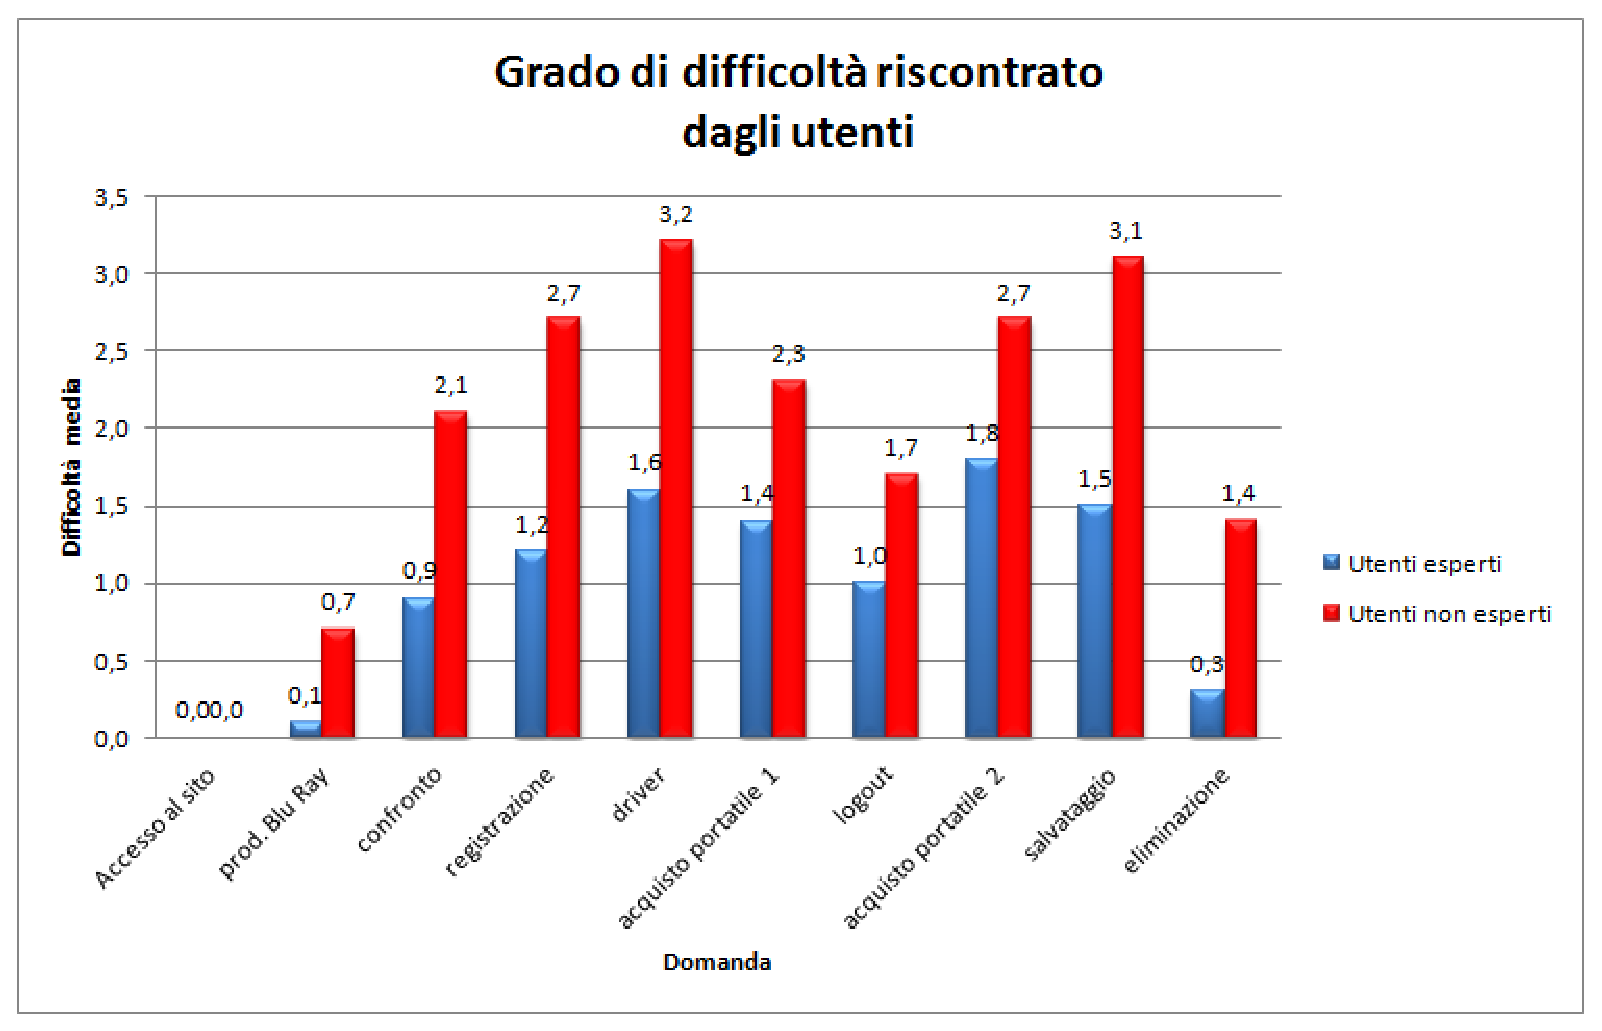
\includegraphics[angle=90,scale=0.75]{figure/grafico_difficolta.eps}
\caption{Grafico media delle difficolt� dei due gruppi d'utenti esaminati}
\label{fig:grafico_difficolta}
\end{figure}
Come evidenziato dal grafico gli utenti esperti considerano i compiti a loro assegnato notevolmente pi� semplici dei loro corrispettivi non esperti. In particolare si evidenzia che la fase di registrazione e di salvataggio della configurazione del secondo portatile risultano avere una valutazione di difficolt� pi� che doppia. Si nota inoltre che alcuni compiti che dovrebbero risultare semplici in realt� non siano tali, come ad esempio la registrazione ed il salvataggio delle proprie impostazioni. Inoltre alcuni utenti hanno valutato la difficolt� di compiti da loro eseguiti fuori tempo massimo o in maniera errata come facile o media.

\subsection*{Valutazione di tempi ed errori}
Esponiamo ora i dati oggettivi raccolti dai due valutatori ossia il tempo impiegato per risolvere i vari task, e gli errori riscontrati per ogni singolo task. Nei seguenti diagrammi si � deciso di mantenere i dati di utenti esperti e non esperti separati, come abbiamo fatto nel paragrafo precedente.


\begin{figure}[!h]
\centering
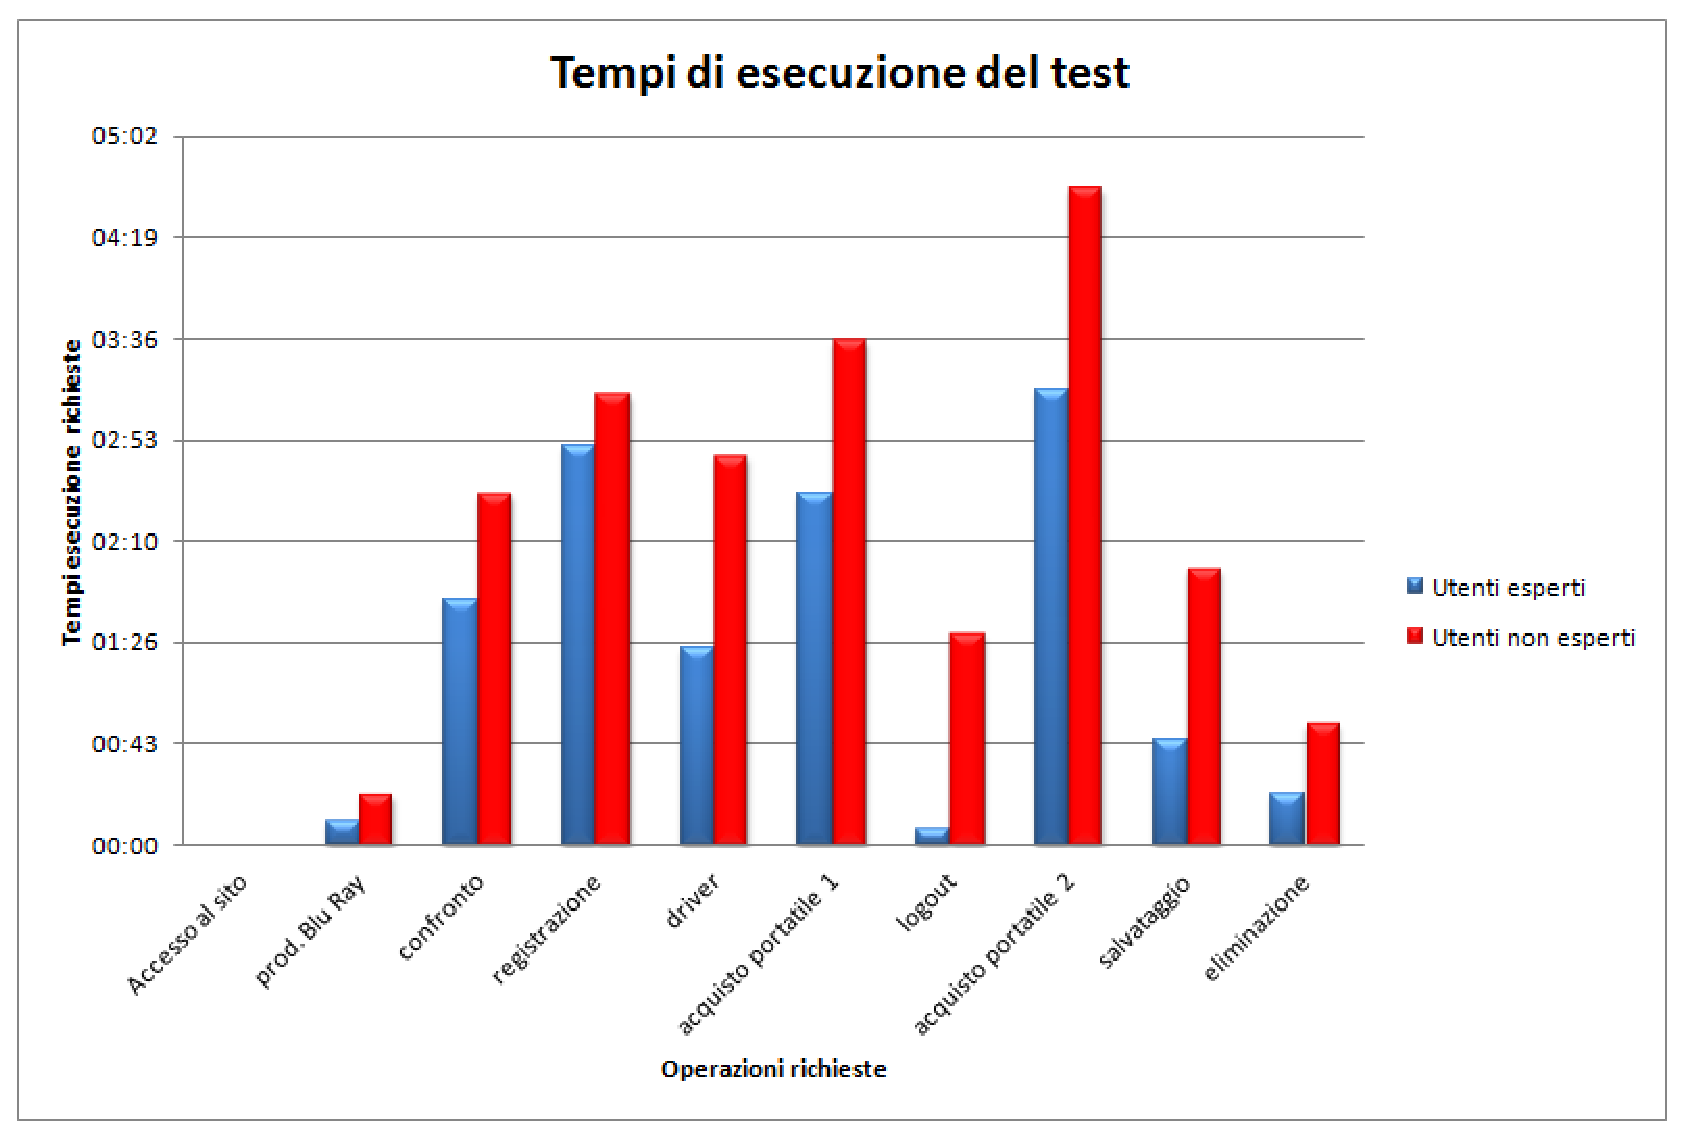
\includegraphics[angle=90, scale=0.75]{figure/grafico_tempi_esecuzione.eps}
\caption{Grafico riportante i tempi di esecuzione delle varie domande del test}
\label{fig:tempi_esecuzione_test}
\end{figure}

Dopo il grafico riguardante i tempi medi passiamo a vedere quello riguardante la quantit� di errori:

\begin{figure}[!h]
\centering
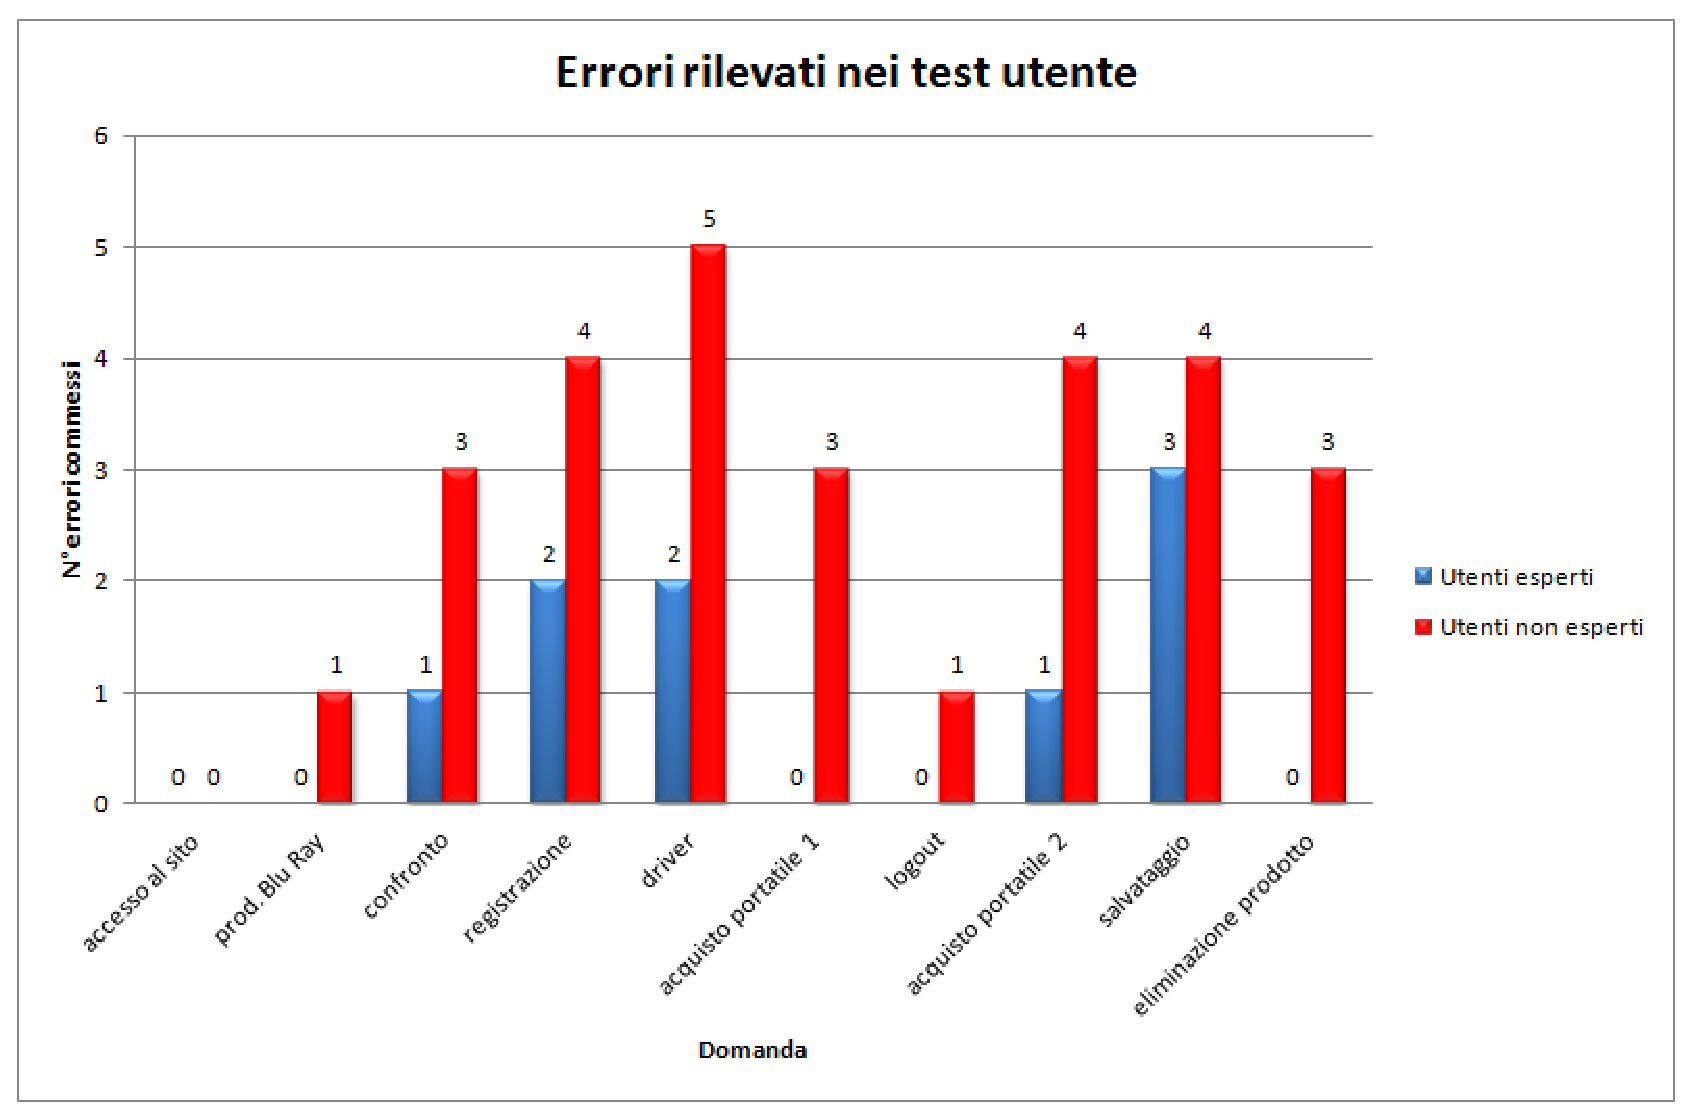
\includegraphics[angle=90, scale=0.75]{figure/grafico_errori_test_utente.eps}
\caption{rafico riportante il numero di errori commessi dagli utenti nella risoluzione dei vari task}
\label{fig:errori_test}
\end{figure}

Dal primo grafico(figura: \ref{fig:tempi_esecuzione_test}) si evince che i tempi impiegati dagli utenti non esperti siano spesso inaccettabili: la ricerca di drivers e software per il computer, cos� come la registrazione hanno comportato lo sforamento del tempo massimo. 
La registrazione � stata particolarmente ostica per gli utenti non esperti, in primo luogo perch� non � immediatamente visibile alcun bottone di registrazione e inoltre la compilazione dei vari form ha spesso costretto a ricompilare pi� volte i campi errati, resettando i campi della password ogni iterazione, introducendo cos� un ulteriore rischio di sbagliare, con conseguente spreco di tempo.\\
Altra operazione che comporta notevole spreco di tempo � la configurazione dei computer da acquistare: non � immediato capire che alcuni passi possono essere saltati e l'utente � portato a seguire sempre il wizard in maniera lineare; spesso anche gli utenti esperti non si sono resi conto del fatto che fossero presenti scorciatoie.\\
Talvolta anche compiti come la rimorzione di elementi dal carrello si � rivelata pi� lenta del previsto: gli utenti meno esperti hanno spesso perso tempo per cercare di cancellare il portatile dal carrello, un ha addirittura effettuato il log-out.\\
Pi� in generale va sottolineato che gli strumenti offerti dal sito spesso sono di poco aiuto, caso eclatante � il form per la ricerca libera, il quale avrebbe dovuto velocizzare diversi task, soprattutto per i pi� esperti, purtroppo spesso i risultati delle ricerche avevano poco o nulla a che vedere con quanto desiderato dagli utenti. Gli help e le sezioni di aiuto non sono mai state usate da nessun utente, nemmeno dai meno esperti quando letteralmente si ``perdevano'' all'interno del sito Dell. Ci� sta ad indicare che essi hanno poca visibilit� all'interno della pagina, oppure non sono dove ci si aspetterebbe.\\
Si nota infine che gli utenti meno esperti oltre ad impiegare pi� tempo dei loro colleghi pi� abituati a navigare facciano anche pi� errori, e in alcuni casi hanno pensato di aver concluso il compito senza invece averlo portato a termine (caso del punto 9, dove era richiesto il salvataggio della configurazione).

